\chapter{Задание \textnumero2}

В листинге~\ref{img:task02} приведён текст второй программы.

\begin{lstlisting}[label=img:task02,caption={Текст второй программы}]
#include <fcntl.h>
#include <errno.h>
#include <stdio.h>
#include <unistd.h>
#include <stdlib.h>
#include <string.h>

int main(void)
{
    char c;
    int flag1, flag2;

    int fd1 = open("alphabet.txt", O_RDONLY);
    if (fd1 == -1)
    {
        fprintf(stderr, "%s: %s\n", "first open alphabet.txt",
                strerror(errno));
        exit(1);
    }
    int fd2 = open("alphabet.txt", O_RDONLY);
    if (fd2 == -1)
    {
        fprintf(stderr, "%s: %s\n", "second open alphabet.txt",
                strerror(errno));
        exit(1);
    }

    do
    {
        if ((flag1 = read(fd1, &c, 1)))
            write(1, &c, 1);

        if ((flag2 = read(fd2, &c, 1)))
            write(1, &c, 1);
    }
    while (flag1 || flag2);

    close(fd1);
    close(fd2);

    return 0;
}
\end{lstlisting}

На рисунке~\ref{img:task02} изображён результат работы второй программы.

\begin{figure}[H]
    \includegraphics[scale=0.5]{images/task02.png}
    \caption{Результат работы второй программы}\label{img:task02}
\end{figure}

В результате двух последовательных вызовов open создаются два разных дескриптора одного файла, который оба раза открывается на чтение, и две записи в системной таблице открытых файлов. Каждому дескриптору соответствует своя текущая позиция в файле.

Таким образом получается, что на каждой итерации цикла два раза происходит чтение одного и того же символа из файла при помощи разных файловых дескрипторов. Следовательно, на каждой итерации цикла выводится два одинаковых символа.

На рисунке~\ref{pdf:task02} изображена связь между созданными дескрипторами.

\begin{figure}[H]
    \centering
    \includegraphics[scale=0.6]{pdf/task02.pdf}
    \caption{Связь между дескрипторами}\label{pdf:task02}
\end{figure}

